\section{Results}
\subsection{Single Phone Model}
Using the architecture detailed in Section 3, we trained the network for 10 epochs
and measured its effectiveness using $k$-fold cross-validation with $k = 10$.
Training/validation data was compiled from the four different diary studies
that used the Nexus 5X.

In normal $k$-fold cross validation, the dataset is randomly partitioned into
$k$-folds. However, we wanted to ensure that for each fold, the validation set
was not biased towards the training set. Specifically, for any state, two samples collected at sequential timesteps
(e.g. sample A at 11:30:00 and sample B at 11:30:30 while the phone was in 
the user's pocket) are likely to be very similar. Then, if one sample 
were partitioned into the training set and the other sample into the validation set, we suspected
that it could be the case that we observe a high validation accuracy, but instead of learning 
a generalizable decision rule, the network may have only learned to remember the class of the sample in the training set 
and regurgitate that class when seeing the very similar other sample in the validation set. 
Our suspicions were confirmed when we observed that the cross-validation accuracy
was $9.22\%$ higher when the dataset was partitioned randomly instead of sequentially.

Accordingly, we decided to partition the data sequentially (i.e. without randomization)
for cross-validation. However, since the diary study data for the Nexus 5X
did not have equal proportions of each class, it was possible for some folds
to have a training set with barely any instances of a class and then validate
on many instances of the same class that the network had limited instances
to train/learn from. To ensure that each fold had comparable training and validation distributions 
for each class, we preprocessed the diary study data before sequentially partitioning it. 
Specifically, we divided the data of each diary study into its 
contiguous segments (e.g. 10:00-11:15, Table or 13:55-14:30, Hand), grouped 
those segments by class, and then concatenated the segments together for each class. The result was four 
homogenous datasets, one of each class, such that for each fold, we could construct
the validation set by aggregating together $\frac{1}{k}$ of each class dataset and then
construct the training set by compiling the remaining $\frac{k - 1}{k}$ of each class dataset.
Within these homogenous class datasets, the data were not randomized but 
kept sequential.

The average accuracy across all folds was $92.06\%$, and the corresponding
confusion matrix is shown in Figure X. The network is able to learn how to 
classify the Table state very accurately, which is understandable given 
the consistent nature of the state (i.e. always in a still, flat position). The states
of Backpack and Pocket were also classified with pretty moderate accuracy,
with the misclassifications likely stemming from the more diverse nature of 
the two states (i.e. the user could have been moving or still when the phone was
in their backpack or pocket). The Hand state was classified with the least accuracy,
and misclassified most often instead as the Backpack state. These misclassifications
likely also stem from the varied positions of the Hand state, as in addition to the user
using the phone actively in their Hand, they may also walk with their phone inactive
in their hand [@Joanna what kind of hand states did you have?]


\begin{table}[h]
\caption{Confusion matrix of the network predictions. Each entry indicates the proportion of
total instances that were predicted as the predicted class by the network and labeled the actual class.}\label{fig:confusion} \centering
\begin{tabular}{| c || c | c | c | c }  
\toprule
\multicolumn{5}{c}{\textit{Actual Class}} \\ \cmidrule{1-5}
\textit{Predicted Class}		&	Backpack    & 	Pocket 	& 	Hand	&	Table \\
\midrule
Backpack			&	0.266 	&	0.005	&	0.024 	&	0.029 \\
Pocket			&	0.016 	&	0.041 	&	0.001 	&	0.001 \\
Hand			&	0.017 	&	0.003 	&	0.035 	&	0.006 \\
Table			&	0.004 	&	0.002 	&	0.002 	&	0.965\\
\bottomrule
\end{tabular}
\end{table}


\subsection{Multiple Phone Models}
We also attempted to validate our networks across different phone models, by training
on data collected by one phone model and then validating on data collected on a 
different phone model. 

However, the same network trained on the Nexus 5X data could unfortunately not be immediately
applied to the Nexus 5 data, as a cursory comparison of the accelerometer data between the two phones 
(while both phones had been on the table) revealed both differing accelerometer readings and readings
that did not equal the expected values of $X = 0g$, $Y = 0g$, and $Z = 9.8g$. Samples, 0.5s long, of 
the two phone's accelerometer data is shown in Figure Y. 

\begin{figure}[t]
\center
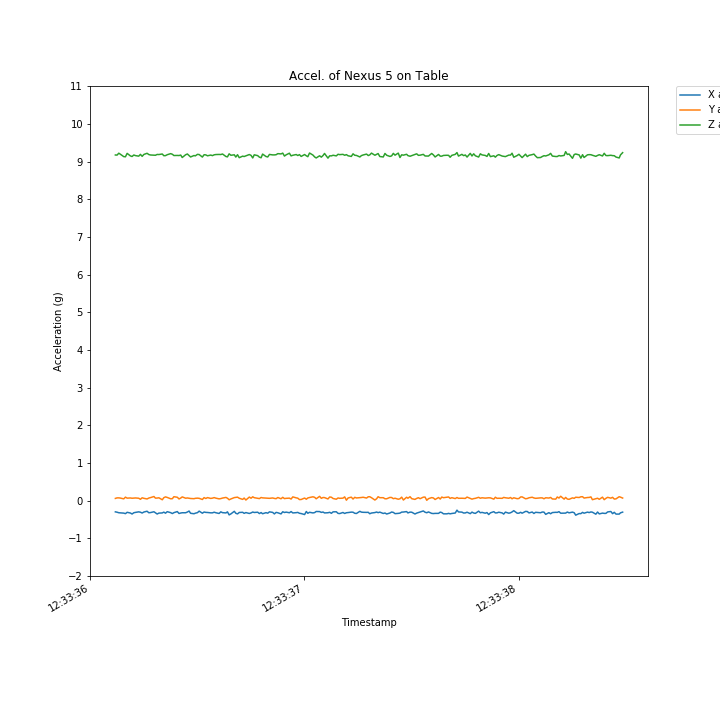
\includegraphics[scale=0.25]{won_table}
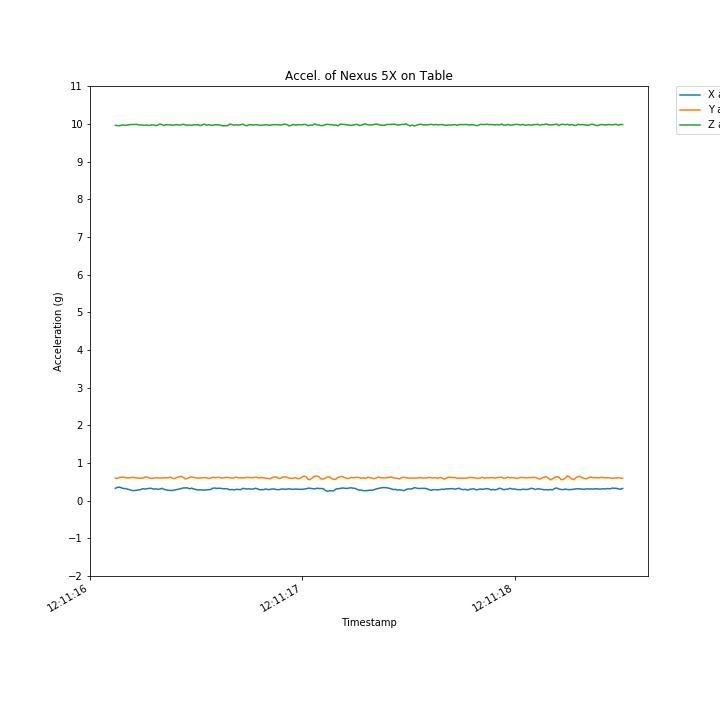
\includegraphics[scale=0.25]{joanna_table}
\caption{Graphs of the acceleration of the Nexus 5 and 5X while on a table (at different times).}
\end{figure}

In order to account for the inconsistent calibrations between the accelerometers of different phone models, we
attempted to recalibrate the accelerometer data for each phone before using it with the network. 
First, to see what type of recalibration model was necessary (e.g. $accel_{calibrated} = accel_{raw} + C$ or
$accel_{calibrated} = K(accel_{raw}) + C$), we taped the Nexus 5 and Nexus 5X together, and then recorded
the phones' accelerations in the four states. Plots of the two phones' accelerations against each other over the same time period
then suggested a linear relationship of the form $accel_{calibrated} = accel_{raw} + C$. 

\begin{figure*}[!h]
\center
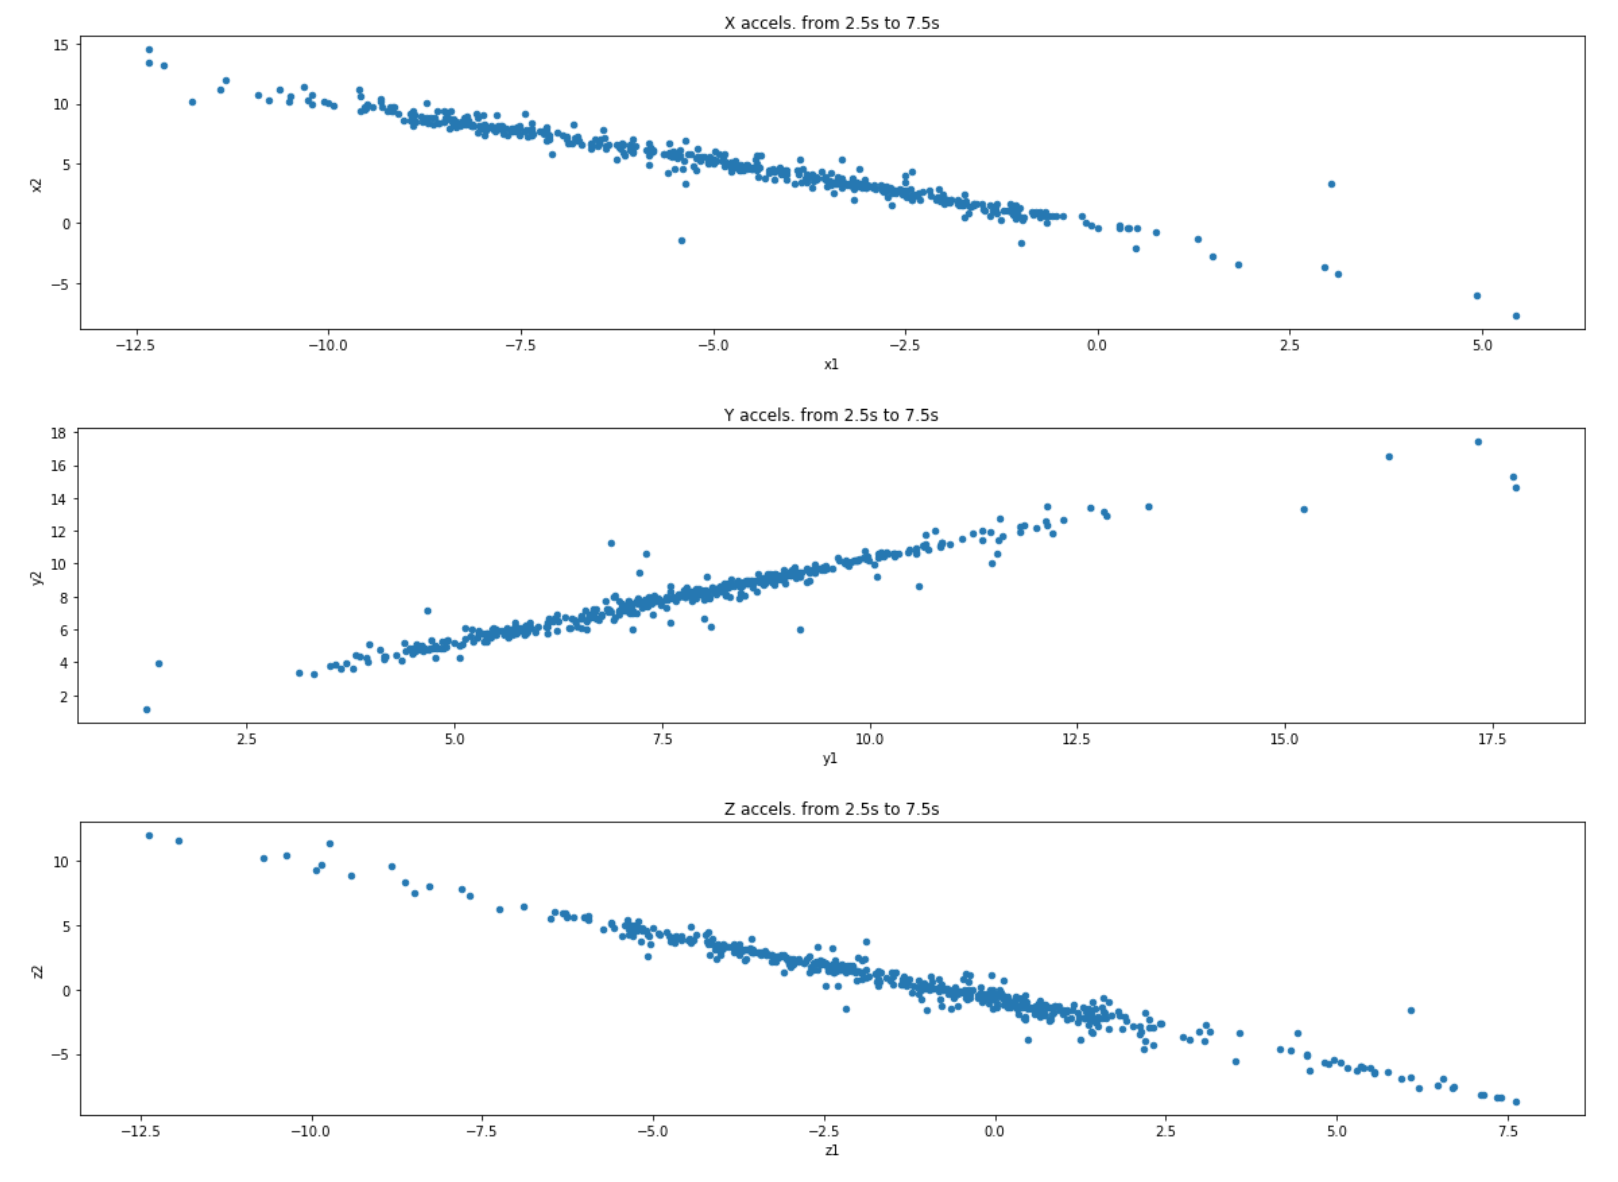
\includegraphics[scale=0.5]{two_phones}
\caption{Graphs of the acceleration of the Nexus 5X (x1/y1/z1) against the Nexus 5 (x2/y2/z2) while taped together over the same period of time.}
\end{figure*}

To find the calibration constants for each phone model, we collected accelerometer
data from when the phone was flat on a table, measured the acceleration in the
$X$, $Y$, and $Z$ directions and then computed the offsets from the expected values of
$0g$, $0g$, and $9.8g$. These offsets were then added to all of the accelerometer data for that phone model.

We applied this calibration process to both the Nexus 5X and Nexus 5 data, and then
trained a network on all of the Nexus 5X data, and validated individually on each of the 
two days of diary study data collected from the Nexus 5.
Nonetheless, even after calibration, results between the two phones were inconclusive. 
On the first diary study with the Nexus 5, our network
had a validation accuracy of only $76\%$, but on the second diary study, our network had a validation
accuracy of $91\%$--an accuracy much more comparable to the cross validation accuracy
demonstrated in the single phone model case. These results suggest that a linear calibration
strategy may be effective, but further investigation is needed for definitive understanding.
